\chapter{基于轨迹数据的群体联合移动模式挖掘}

\section{引言}
本章通过对大规模移动轨迹的系统分析，旨在设计高效且可扩展的算法框架，用于识别在特定时间区间内频繁共同出现在相邻空间位置，且在多个时间点存在联合移动的对象集合，即特定群体联合移动模式。该问题有助于为城市规划、交通管理以及社会行为研究等应用场景提供更加深入和精细化的决策支持。

为实现上述目标，本章从数据建模、索引结构设计与算法优化等多个层面展开研究。首先，对特定群体模式检测问题进行形式化定义，明确问题输入、输出及约束条件，并系统分析其在大规模数据环境下面临的计算复杂性与存储开销挑战；其次，结合时空数据挖掘技术，构建适用于大规模轨迹数据的高效索引结构，以支持高性能的候选模式生成与验证过程。在研究背景方面，调研了联合移动模式搜索与轨迹聚类领域的代表性工作，总结其在模式表达能力、计算效率与扩展性方面的优势与不足，从而引出本章研究的核心问题与技术挑战。在问题描述层面，本章依次给出了移动对象及其轨迹的形式化定义，刻画了协同行为的时间持续约束以及空间共现条件，并在此基础上提出了一个更加简化且具有实际意义的伴随群体发现问题定义。

总体而言，大规模性、模式定义的灵活性、算法效率要求以及数据动态变化特征共同构成了该问题的技术难点，也对算法框架设计与系统实现提出了更高要求。针对伴随群体发现问题，首先设计了一种精确求解算法，随后提出了一种新颖的社区感知聚类模型，返回近似解，以有效缩减搜索空间并提升候选群体的质量。基于两个真实世界数据集开展了全面的实验评估，实验结果表明，所提出的社区感知算法能够在用户可交互时间范围内，从大规模轨迹数据中高效发现伴随群体，验证了在实际应用场景中的可行性。

\subsection{研究背景与意义}

随着位置追踪设备，如车载导航系统和智能手机以及 GPS 智能服务的持续普及，轨迹数据的规模呈现爆炸式增长。作为时空数据挖掘中的一项核心任务，联合移动模式挖掘问题已受到广泛关注。一般而言，联合移动模式描述一组在一段时间内在空间上保持接近的对象集合。围绕这一问题，研究者提出了多种具有代表性的模式定义，包括 flock~\cite{DBLP:conf/gis/VieiraBT09,DBLP:journals/jidm/TanakaVK16}、convoy~\cite{DBLP:journals/pvldb/JeungYZJS08}、swarm~\cite{DBLP:journals/pvldb/LiDHK10}、group~\cite{DBLP:journals/dke/WangLH06}、platoon~\cite{DBLP:journals/dke/LiBK15} 以及 gathering~\cite{DBLP:conf/icde/ZhengZYS13,DBLP:journals/tkde/ZhengZYSZ14} 等。这些模式在时间连续性约束、空间密度约束以及成员稳定性等方面各有侧重，共同构成了联合移动模式研究的理论基础。

在诸多实际应用中，高效且准确地从移动对象轨迹中发现联合移动模式具有重要意义。例如，在拼车推荐与出行规划中，可以通过识别稳定的同行群体，使其共同出发或考虑彼此对交通的影响等，从而提升资源利用率；在交通拥堵缓解中，可通过及早发现道路上的高密度移动群体来规避潜在拥堵；在新冠病毒等传染病的暴露与风险分析中，可辅助识别潜在高风险接触群体~\cite{imo,DBLP:journals/information/AlarabiBHA21}；此外，在移动行为分析与异常轨迹检测~\cite{DBLP:conf/icde/Liu0CB20} 等任务中，群体模式挖掘同样发挥着关键作用。

然而，如何在保证模式表达能力的同时提升计算效率，成为该领域亟需解决的重要问题。现有研究大多基于移动对象随时间演化的完整轨迹设计搜索算法。这类方法通常在每一个时间快照上执行聚类或密度计算，以判断对象之间的空间邻近关系。当联合移动模式在时间上不稳定，即对象可能暂时离开群体后又重新加入时，算法需要反复进行候选生成与验证，计算代价显著增加。尤其是在实时或近实时应用场景中，对所有时间快照进行全量聚类将带来极高的时间开销。此外，主流方法多采用“过滤–精炼”的处理框架，在过滤阶段通过建立时空索引排除不可能的数据对象，仅保留可能的候选群体，再在精炼阶段逐一验证其有效性。随着轨迹数据规模的持续增长，候选数量呈指数级膨胀，导致算法性能显著下降，难以满足大规模与在线分析的需求。



\subsection{研究内容与挑战}
在现实应用中，尤其是在公共安全紧急预警与传染病防控等对时效性要求极高的场景下，及时获得最新的联合移动结果至关重要。因此，联合移动模式挖掘任务往往需要以连续或增量的方式执行。这不仅要求算法在时间复杂度上具备良好的可扩展性，还要求其在模式定义上具有一定的灵活性，以适应动态变化的移动行为。然而，现有群体模式定义及其对应方法在同时兼顾模式表达能力与计算效率方面仍存在明显不足，难以在大规模数据环境中实现高效、稳定的持续挖掘。

为了解决上述问题，本文提出了一种联合移动模式概念——伴随群体。相较于已经存在的传统的联合移动模式定义，伴随群体的约束更加宽松且更具实用性。具体而言，一个伴随群体由至少 $m$ 个移动对象组成，这些对象需要在至少 $k$ 个时间段内在空间上保持接近（例如，两两距离不超过预定义的距离阈值 $\epsilon$），并允许对象在时间维度上暂时离开群体而不破坏整体模式的有效性。基于该模式定义，进一步形式化提出了伴随群体发现问题。给定一组移动对象及其轨迹数据，伴随群体发现问题旨在在用户可交互时间范围内高效发现所有满足条件的伴随群体。此外，在问题设定中，若某一对象能够同时参与多个伴随群体，则将其归属于成员规模最大的伴随群体，以保证群体划分结果的确定性与可解释性。伴随群体发现问题问题具有广泛的应用前景，可服务于交通监测与管理、疫情防控、公共安全预警以及群体行为分析等多种实际场景，为大规模时空数据环境下的群体行为挖掘提供一种高效且可扩展的解决方案。

\begin{figure}[htbp]
    \centering
    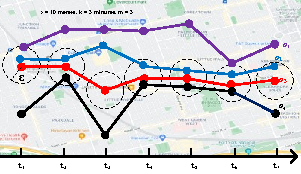
\includegraphics[width=1\textwidth]{fig/section4/group companion.pdf}
    \caption{伴随群体发现问题示例}
    \label{cm_fig:intro}
\end{figure}

\begin{example}[伴随群体发现问题示例]
图~\ref{cm_fig:intro}给出了一个具体示例以直观说明伴随群体的判定过程。设 $o_1, o_2, o_3, o_4$ 为四个移动对象，且所有对象以固定采样频率每分钟上报一次位置信息。图~\ref{cm_fig:intro} 展示了这四个移动对象在时间区间 $[t_1, t_7]$ 内的轨迹变化情况。设空间距离阈值为 $\epsilon = 10$ 米，联合移动的最小持续时间阈值为 $k = 3$，群体规模阈值为 $m = 3$。首先，从对象两两关系的角度进行分析。可以观察到，对象 $o_2$ 与 $o_3$ 在时间集合 $T = \{t_1, t_2, t_4, t_5, t_6, t_7\}$ 内始终满足两两距离不超过 $\epsilon$ 的约束，即在这些时间点保持空间接近关系。由于 $|T| = 6$，显著超过持续时间阈值 $k$，因此 $o_2$ 与 $o_3$ 构成一个满足条件的联合移动对。同理，$o_3$ 与 $o_4$ 在不少于 $k$ 个时间点内保持空间邻近关系，也可以构成一个联合移动对。在此基础上，进一步考察多对象群体关系。可以发现，在时间点 $\{t_2, t_4, t_5, t_6\}$ 上，对象 $o_2, o_3, o_4$ 的两两距离均不超过 $\epsilon$，即它们在这些时间点形成一个空间上连通且满足密度约束的三元对象集合。由于该时间集合的规模不少于持续时间阈值 $k$，且群体规模 $|g| = 3$ 满足最小规模阈值 $m$，因此将 $g=\{o_2, o_3, o_4\}$ 判定为一个有效的伴随群体。需要注意的是，对象 $o_1$ 仅在 $t_1$ 和 $t_6$ 与 $o_2$ 短暂接近，其满足距离约束的时间点数量不足以达到持续时间阈值 $k$，且未能与其他对象形成稳定的多对象联合移动模式。因此，$o_1$ 既无法与其他对象构成有效的联合移动对，也不能参与任何满足条件的伴随群体。该示例说明，伴随群体的判定不仅依赖于空间邻近关系，还同时受到时间持续性与群体规模约束的共同影响，从而能够更全面地刻画移动对象之间的协同行为特征。
\end{example}
为了高效解决伴随群体发现问题，系统在算法设计与工程实现层面面临多方面的关键技术挑战，这些挑战既来源于数据本身的规模与动态特性，也源于模式定义的复杂性与计算代价。具体而言，主要包括以下几个方面：

\begin{itemize}
    \item \textbf{大规模数据处理：}在真实应用场景中，轨迹数据通常来源于海量移动对象，例如车辆、移动终端或各类传感设备，其数据规模可能达到千万级甚至更高。轨迹数据不仅记录频繁，而且具有高维度与强相关性特征，使得存储与计算开销显著增加。如何在如此庞大的数据规模下实现高效的数据组织、索引构建与查询处理，尤其是在需要实时或近实时发现群体模式的场景中，成为首要挑战。这不仅要求算法具备良好的时间复杂度和可扩展性，还需要设计紧凑的空间组织结构与高效的内存管理策略，以降低存储成本并减少 I/O 开销。

    \item \textbf{模式定义的灵活性：}不同应用场景对群体模式的语义需求存在差异。例如，有的应用更关注空间邻近性，有的强调时间持续性，还有的关注成员规模或运动一致性等约束条件。因此，如何构建一个既支持多种群体模式表达，又能够灵活调整参数（如距离阈值、持续时间阈值与最小群体规模）的统一算法框架，是实现方法广泛适用性的关键。同时，该框架在增强表达能力的同时，必须避免因模式定义过于复杂而导致搜索空间急剧膨胀，从而影响整体计算效率。

    \item \textbf{准确性与效率的平衡：}群体模式发现通常涉及复杂的时空约束匹配、多对象关系维护以及候选结构验证等操作。若直接采用精确枚举算法，往往需要在大量时间快照上反复执行聚类或连通性检测，计算代价极高。因此，如何在保证结果准确性的前提下，通过有效的剪枝策略、搜索空间压缩技术、分层索引机制或近似计算方法减少不必要的候选生成与验证，是提升系统性能的核心问题。尤其在数据规模持续增长的背景下，算法必须在结果质量与运行效率之间取得合理且可控的权衡。

    \item \textbf{动态性的处理：}轨迹数据具有天然的动态特征，移动对象的位置与行为随时间持续变化。在流式或持续更新的数据环境中，新轨迹不断到达，历史数据逐渐失效，群体结构也随之演化。若每次更新都重新对全部历史数据进行计算，将带来难以接受的时间开销。因此，如何设计支持增量更新或滑动窗口处理机制的算法，在无需重复计算全部数据的前提下高效维护群体模式结果，是保证系统实时性、稳定性与可扩展性的关键技术挑战。
\end{itemize}

\subsection{研究成果与贡献}
综上所述，大规模数据处理需求、模式定义的灵活性要求、算法效率约束以及数据动态演化特征，共同构成了伴随群体发现问题的核心技术难点，也对整体算法框架设计与系统实现提出了更高要求。针对伴随群体发现问题，本文从精确算法设计与高效近似算法设计两个层面展开研究。

首先，设计了一种精确搜索算法。该算法基于严格的时空约束判定机制，对候选对象对及候选群体进行精确验证，能够保证结果的完备性与准确性。然而，由于需要在多个时间维度上进行精细化匹配与验证，其计算代价相对较高，更适用于离线分析或数据规模适中的场景。

为进一步提升算法效率并满足实时或近实时应用需求，本文额外提出了一种社区感知的近似搜索算法。该算法在保证结果质量可控的前提下，通过近似计算与结构化聚类方法显著压缩搜索空间，从而在严格的效率约束下有效解决伴随群体发现问题，实现准确性与效率之间的平衡。

近似算法主要包括两个阶段：近似联合移动对搜索阶段与社区感知群体发现阶段。在近似联合移动对搜索阶段，首先采用基于网格划分的空间离散化方法，将每个轨迹位置映射为对应的网格单元编号，从而将连续轨迹转换为离散的网格单元编号序列表示。随后，通过计算不同轨迹之间的公共编号数量来快速估计其潜在的联合移动程度，从而生成候选的近似联合移动对。该过程有效避免了在原始连续空间中进行高代价的距离计算。在社区感知群体发现阶段，将生成的联合移动对视为图结构中的边，并利用 SCAN 算法~\cite{DBLP:conf/kdd/XuYFS07} 进行结构化聚类，以识别具有高内聚性和清晰社区边界的对象集合。通过引入社区结构约束，算法能够在保证群体结构合理性的同时，进一步降低无效候选的数量，从而提升整体运行效率。本文算法实现已开源发布\footnote{https://github.com/Like-China/gathering\_mining.git}，以便于后续研究复现与扩展。

本文的主要贡献总结如下：
\begin{itemize}
    \item 提出了伴随群体这一联合移动模式定义。该定义相较于传统模式更加宽松且具备更强的适应性，尤其适用于需要持续结果更新与快速响应的应用场景，例如传染病传播监测与公共安全紧急风险预警。
    \item 设计并实现了一种精确搜索算法以及一种社区感知的近似搜索算法，系统性地解决了伴随群体发现问题在准确性与效率之间的权衡难题。
    \item 基于两个真实世界数据集开展了全面的实验评估。实验结果表明，所提出的社区感知算法能够在用户可交互时间范围内，从大规模轨迹数据中高效发现伴随群体，验证了方法在实际应用场景中的有效性与实用价值。
\end{itemize}

本文其余部分组织结构如下。第~\ref{cm_sec:problem} 节首先形式化给出问题定义，并介绍相关的符号说明与必要的预备知识，为后续算法设计奠定理论基础。第~\ref{cm_sec:exact} 节在此基础上提出一种精确算法，详细阐述其核心思想、实现流程以及时间复杂度分析。第~\ref{cm_sec:approximate} 节进一步给出一种社区感知的高效近似算法，通过结构压缩与候选剪枝策略提升算法的可扩展性，并分析其性能优势与适用场景。第~\ref{cm_sec:exp} 节基于真实世界轨迹数据开展系统实验，从有效性与效率两个方面对所提方法进行全面评估与对比分析。最后，第~\ref{cm_sec:conclusion} 节对全文进行总结，并展望未来的研究方向。

\section{问题定义}
\label{cm_sec:problem}

本节介绍所需的基础概念，并给出问题的形式化定义。给定一组移动对象，依次定义移动对象及其轨迹、协同行为持续时间、协同行为对、伴随群体以及伴随群体发现问题。本章所使用的主要符号及其解释如表\ref{cm_tab:notation}所示。

\begin{table}[htbp]
    \centering
    \setlength{\tabcolsep}{8pt}% column separation
    \caption{主要符号解释}
    \label{cm_tab:notation}
    \renewcommand{\arraystretch}{1}%row space 
    \begin{tabular}{ll}
        \hline
		\bfseries 符号 & \bfseries 解释 \\
        \hline
        $o$ & 一个移动对象\\
        $O$ & 一组移动对象集合\\
        $s$ & 一个采样位置点\\
        $\tau$ & 一条轨迹 \\
        $\mathcal{T}$ & 一组轨迹集合\\
        $t$ & 某个时刻\\
        $\epsilon_s$/$\epsilon_t$ & 空间距离阈值/时间距离阈值\\
        $k$ & 协同行为持续时间阈值\\
        $m$ & 最小群体规模阈值 \\
        $g$ &一个伴随群体\\
        $\mathcal{G}$ & 一组伴随群体 \\
        \hline
    \end{tabular}
\end{table}

\begin{definition}[移动对象及其轨迹]
一个移动对象 $o$ 由其轨迹 $\tau=\{s_1,\ldots,s_n\}$ 表示，其中轨迹是一个有限的、按时间顺序排列的离散时空点序列。该序列由位置追踪设备从对象 $o$ 的真实运动轨迹中采样获得。

为简化描述，使用 $s_i=([x,y],t)$ 表示二维空间中的一个离散采样位置点，其中 $[x,y]$ 表示空间坐标，$t$ 表示该位置被记录时对应的时间戳。对于一组移动对象 $O$，记其轨迹集合为 $\mathcal{T}=\{\tau_1,\ldots,\tau_{|O|}\}$，其中 $\tau_i$ 为对象 $o_i$ 的轨迹。本文对移动对象及轨迹的建模方式与已有研究保持一致~\cite{DBLP:conf/ijcai/LiCSWLK022,DBLP:conf/icde/RanuPTDR15,DBLP:conf/sigmod/SuZWHZ13}。
\end{definition}

\begin{definition}[协同行为持续时间]
设 $o_i$ 与 $o_j$ 为两个移动对象。当 $o_i$ 与 $o_j$ 之间的空间距离小于等于给定的空间距离阈值 $\epsilon_s$，且对应时间戳之差不超过给定的时间距离阈值 $\epsilon_t$ 时，称二者在该时刻处于协同行为状态。对象 $o_i$ 与 $o_j$ 的协同行为持续时间定义为所有满足上述条件的时间长度之和。
\end{definition}

\begin{definition}[协同行为对]
设 $\tau_i$ 与 $\tau_j$ 分别为对象 $o_i$ 与 $o_j$ 的轨迹。给定$k$ 为协同行为持续时间阈值，若 $\tau_i$ 与 $\tau_j$ 之间的协同行为持续时间不少于给定阈值 $k$，则称对象 $o_i$ 与 $o_j$ 构成一个协同行为对。
\end{definition}

\begin{definition}[伴随群体]
给定一组移动对象 $\mathcal{O}=\{o_1,o_2,\ldots,o_{|\mathcal{O}|}\}$ 以及最小群体规模阈值 $m$，若对象子集 $g\subseteq \mathcal{O}$ 满足以下两个条件，则称 $g$ 为一个伴随群体：
\begin{enumerate}
    \item $|g|\geq m$；
    \item 对任意两个对象 $o_i,o_j\in g$，$o_i$ 与 $o_j$ 均构成协同行为对。
\end{enumerate}
\end{definition}

\begin{definition}[伴随群体发现问题]
给定一组移动对象 $\mathcal{O}$，伴随群体发现问题旨在从 $\mathcal{O}$ 中发现一组伴随群体 $\mathcal{G}$，并满足对任意两个群体 $g_i, g_j\in\mathcal{G}$，均有 $g_i\cap g_j=\emptyset$。
\end{definition}

\section{精确搜索算法}
\label{cm_sec:exact}

本节提出一种用于发现伴随群体的精确求解方法——精确联合移动算法（\underline{E}xact \underline{S}earch with \underline{E}xact \underline{C}o-\underline{M}ovement \underline{C}omputation，简称 ES-ECMC）。该算法对所有候选对象组合进行精确验证，从而保证结果的完备性与正确性。

ES-ECMC 算法整体上包含三个核心步骤。首先，给定输入数据，即一组移动对象轨迹集合，通过精确的时空约束计算枚举并识别所有满足持续时间阈值 $k$ 的联合移动对；其次，以这些联合移动对为基础，构建对象之间的关联结构，并采用增量扩展策略逐步生成满足条件的伴随群体候选；最后，在所有生成的候选集合中，依据成员规模优先的原则筛选出不可扩展且规模最大的伴随群体作为最终输出结果。该三阶段流程分别对应“协同行为对发现—伴随群体候选集合扩展—结果筛选”三个层次，层层递进，从而实现对搜索空间的系统化遍历与剪枝。在介绍具体流程之前，首先给出伴随群体候选的形式化定义，以便后续算法描述与性质分析。

\begin{definition}[伴随群体候选]
一个伴随群体候选 $g'$ 是一个对象集合，满足其中任意两个对象均可以构成一个联合移动对。若存在至少一个集合外的对象 $o \notin g'$，使得扩展后的集合 $g' \cup \{o\}$ 仍然满足上述条件，则称 $g'$ 可以通过加入对象 $o$ 进行扩展；否则，称 $g'$ 为不可扩展的伴随群体候选。
\end{definition}


\begin{algorithm}[htbp]
    \caption{ES-ECMC}
    \label{cm_alg:S-ECMC}
    \Input{轨迹集$\mathcal{T}=\{\tau_1,\tau_2,\ldots,\tau_{|\mathcal{O}|}\}$;\newline
    空间距离阈值 $\epsilon_s$;\newline
    时间距离阈值 $\epsilon_t$;\newline
    群体规模阈值 $m$;\newline
    联合移动持续时间阈值 $k$。
    }
    
    \Output{一组满足定义约束的精确的伴随群体集合 $G$。}
    
    \BlankLine
    初始化：$P \leftarrow \emptyset$;\tcp*[f]{有效轨迹对集合}

    初始化：$G_c \leftarrow \emptyset$;\tcp*[f]{候选群体集合}

    初始化：$G \leftarrow \emptyset$;\tcp*[f]{最终结果集合}
    
    \BlankLine
    \For(\tcc*[f]{生成有效轨迹对}){$i = 1$ \KwTo $|\mathcal{T}|$}{
        \For{$j = i+1$ \KwTo $|\mathcal{T}|$}{
            \If{$|\tau_i \cap \tau_j| \ge k$}{
                $P \leftarrow P \cup \{(\tau_i,\tau_j)\}$;
            }
        }
    }
    
    \BlankLine
    \ForEach(\tcc*[f]{扩展候选群体}){$(\tau_i,\tau_j) \in P$}{
        $g_i \leftarrow \{\tau_i,\tau_j\}$;
    
        \ForEach{$(\tau_i,\tau_k) \in P$}{
            \If(\tcc*[f]{两两有效且所有成员均在 $g_i$ 中})
            {$\forall \tau_p \in g_i,\; (\tau_k,\tau_p) \in P$}{
                $g_i \leftarrow g_i \cup \{\tau_k\}$;
            }
        }
    
        \If(\tcc*[f]{群体规模约束}){$|g_i| \ge m$}{
            $G_c \leftarrow G_c \cup \{g_i\}$;
        }
    }
    
    \BlankLine
    $G \leftarrow select\_max(G_c)$;\tcp*[f]{选择最大或最优群体}
    
    \Return $G$;
\end{algorithm}


下面将详细介绍 ES-ECMC 算法的整体流程与核心思想。算法~\ref{cm_alg:S-ECMC} 给出了 ES-ECMC 的完整伪代码描述。该算法以一组轨迹数据 $\mathcal{T}$ 作为输入，同时给定空间距离阈值 $\epsilon_s$、时间距离阈值 $\epsilon_t$、最小群体规模阈值 $m$ 以及联合移动持续时间阈值 $k$。算法的输出为一组满足定义约束的伴随群体集合
$G=\{g_1,g_2,\ldots\}$，其中每个 $g_i \subseteq \mathcal{T}$，表示由若干移动对象轨迹构成的一个伴随群体。在实现层面，使用一个集合 $P$ 存储所有满足持续时间阈值 $k$ 的协同行为对，用以刻画对象之间的两两联合移动关系 （第1行）；同时，使用一个集合 $G_c$ 存储在搜索过程中生成的伴随群体候选 （第2行）。通过先构建联合移动对集合 $P$，再基于 $P$ 进行增量式候选扩展与验证，算法能够系统地遍历可能的对象组合，并通过可扩展性判定与规模约束进行有效剪枝，从而最终得到满足条件的伴随群体集合 $G$ （第3行）。该算法包含3个主要步骤：枚举联合移动对，生成伴随群体候选，以及选择伴随群体。

    \underline{步骤 1：}（枚举联合移动对）

    对于任意一对移动对象 $o_i, o_j \in \mathcal{O}$，计算其轨迹中任意两个采样位置
    $s \in \tau_i$ 与 $s' \in \tau_j$ 之间的精确距离。若空间距离与时间距离分别不超过阈值 $\epsilon_s$ 与 $\epsilon_t$，则将其联合移动持续时间 $|\tau_i \land \tau_j|$ 累加 1。具体而言，对于每一对对象 $\langle o_i,o_j\rangle$，当其累计的联合移动持续时间不少于阈值 $k$ 时，将其视为一个联合移动对\footnote{在上下文清晰的情况下，使用 $(o_i,o_j)$ 或 $(\tau_i,\tau_j)$ 表示一个联合移动对。}。当所有对象对均被评估完成后，该步骤结束（第 4--7 行）。
    
    \smallskip
    \underline{步骤 2：}（生成伴随群体候选）
    
    在获得所有联合移动对之后，基于这些联合移动对以增量方式生成伴随群体候选。具体而言，首先选择一个以轨迹 $\tau_i$ 为起点的联合移动对，例如 $\langle \tau_i,\tau_j\rangle$，然后考察所有与其共享对象 $o_i$ 的联合移动对 $\langle \tau_i,\tau_k\rangle$。初始群体记为 $g_i=\{\tau_i,\tau_j\}$。若 $\tau_k$ 与 $g_i$ 中的所有成员均构成联合移动对，则将 $\tau_k$ 加入 $g_i$。当 $g_i$ 仍可扩展时，重复上述扩展过程。若 $|g_i| \ge m$，则将其加入候选集合 $G_c$。随后选择新的联合移动对作为初始群体并继续扩展。当所有联合移动对均被访问并作为初始群体尝试扩展后，该步骤结束（第 8--14 行）。
    
    \smallskip
    \underline{步骤 3：}（选择伴随群体）
    
    在获得所有候选群体之后，从中选取成员规模最大的伴随群体作为最终结果。具体而言，若某个对象同时属于多个候选群体，则仅保留其中成员规模最大的一个。该步骤在遍历完所有候选群体后结束（第 15 行）。
    
    \begin{example}[ES-ECMC算法示例]
    再次考虑图~\ref{cm_fig:intro} 中的示例。假设首先选择联合移动对 $\langle o_2,o_3\rangle$ 进行扩展。显然，联合移动对 $\langle o_2,o_4\rangle$ 与 $\langle o_2,o_3\rangle$ 共享对象 $o_2$，且对象 $o_2,o_3,o_4$ 两两之间均可形成联合移动对。因此，将 $g'=\{o_2,o_3,o_4\}$ 视为一个伴随群体候选。由于对象 $o_1$ 无法与 $g'$ 中的任一对象形成联合移动对，$g'$ 不可进一步扩展。接着，由于 $|g'|$ 不小于预设的群体规模阈值 3，将 $g'$ 加入候选集合 $G_c$。最终，由于 $g'$ 具有最大的成员规模，从 $G_c$ 中选取 $g'$ 并将其加入结果集合 $G$。
    \end{example}



    \begin{theorem}[ES-ECMC 算法时间复杂度]
    ES-ECMC 算法的时间复杂度为 $O(|\mathcal{T}|^2 \times |\tau|^2)$，其中 $|\mathcal{T}|$ 表示移动对象或轨迹的数量，$|\tau|$ 表示单条轨迹的平均长度，即采样位置数。
    \end{theorem}
    
    \begin{proof}
    ES-ECMC 的主要时间开销来自三个阶段。
    
    首先，在枚举所有联合移动对时，需要对任意一对轨迹 $\tau_i,\tau_j \in \mathcal{T}$ 进行逐点比较。对于每一对轨迹，需计算其所有采样点对之间的空间距离与时间距离，时间复杂度为 $O(|\tau|^2)$。由于轨迹对的数量为 $O(|\mathcal{T}|^2)$，因此该阶段的总体时间复杂度为
    \[
    O(|\mathcal{T}|^2 \times |\tau|^2)。
    \]
    
    其次，在生成伴随群体候选阶段，对于共享同一对象的联合移动对（例如 $\langle o_i,o_j\rangle$ 与 $\langle o_i,o_k\rangle$），需要判断其是否能够构成伴随群体候选，并在满足条件时进行扩展。该过程本质上是在联合移动对构成的图结构上进行增量式团扩展。最少情况下（例如不存在任何共享对象的联合移动对），该阶段仅需线性扫描联合移动对集合，时间复杂度为 $O(|\mathcal{T}|)$；在最坏情况下，若任意两个对象之间均可形成联合移动对，则候选生成过程可能涉及 $O(|\mathcal{T}|^2)$ 次组合与验证操作。然而，该阶段的复杂度上界仍然不超过前一阶段的 $O(|\mathcal{T}|^2 \times |\tau|^2)$。
    
    最后，在候选集合 $G_c$ 中选择最终伴随群体时，仅需遍历所有候选并进行规模比较，时间复杂度为 $O(|G_c|)$。由于 $|G_c| < |\mathcal{T}|^2$，且通常远小于前两阶段的计算规模，因此该阶段不会改变整体复杂度阶。
    综上所述，ES-ECMC 算法的总体时间复杂度由联合移动对枚举阶段主导，为
    \[
    O(|\mathcal{T}|^2 \times |\tau|^2)。
    \]
    \end{proof}


\section{基于近似协同行为计算的社区感知搜索}
\label{cm_sec:approximate}

尽管 ES-ECMC 精确算法直观且能够保证结果的精确性，但其较高的计算开销使其难以直接应用于大规模实际场景，尤其是在移动对象数量极大的情况下。其主要性能瓶颈在于需要通过精确计算协同行为持续时间来枚举所有协同行为对，该过程涉及大量轨迹间的逐点比较操作，时间代价高昂。为提升算法效率，本文提出一种基于社区感知的搜索算法，并结合近似协同行为计算策略，即 \underline{C}ommunity-aware \underline{S}earch with \underline{A}pproximate \underline{C}o-\underline{M}ovement \underline{C}omputation（简称 CS-ACMC）。该方法在保证较高结果质量的同时，显著降低了计算复杂度。CS-ACMC 算法主要包含两个阶段：（1）近似协同行为对搜索阶段，通过构建轨迹的紧凑表示并进行快速相似性筛选，以高效识别潜在的协同行为对；（2）基于社区感知的聚类阶段，在所构建的对象关系图上挖掘结构紧密的对象子集，从而获得伴随群体。接下来，将依次介绍近似协同行为对搜索策略以及社区感知聚类算法的具体设计。

\subsection{近似协同行为对搜索}

在该阶段中，提出了一种高效的协同行为对搜索方法，用于计算两个对象轨迹之间协同行为持续时间的近似值。所生成的近似协同行为对将作为后续社区感知聚类阶段的输入，从而高效地发现伴随群体。该阶段包含两个子步骤：生成轨迹网格编号序列，以及搜索近似协同行为对。

\subsubsection{轨迹网格编号序列生成}

该方法受到群体（flock）圆形结构思想的启发 \cite{DBLP:journals/pvldb/JeungYZJS08}。首先将底层时空域进行离散化处理：在空间维度上，将二维欧氏空间划分为边长相等的网格单元；在时间维度上，将时间轴划分为等长的时间片。因此，对于对象轨迹中的每一个数据点（位置）$s=([x,y],t)$，均可映射为一个网格编号，记为
$o(s)=f(x,y,t)$，
其中 $f(\cdot)$ 为单射函数，用于将三维离散坐标唯一映射为一个整数标识。由此，轨迹 $\tau$ 可表示为对应的网格编号序列：
$
O(\tau)=\{o(s_1),\ldots,o(s_{|\tau|})\}
$。图 \ref{cm_fig1:cell_partition} 展示了空间与时间维度的划分方式以及轨迹网格编号序列的生成过程。假设空间被划分为 $5\times 4$ 个网格单元，每个单元边长为 10 米，时间维度被划分为 3 个时间片，每个时间片长度为 10 秒。给定两条轨迹 $\tau_1$ 和 $\tau_2$，其位置分别落入单元
$\{([0,0],0), ([3,1],1), ([2,1],2)\}$。基于上述划分方式，定义单射函数为
$o(s)=f(x,y,t)=t\times(5\times4)+y\times5+x$，
其中 $x\in\{0,1,2,3,4\}$，$y\in\{0,1,2,3\}$，$t\in\{0,1,2\}$。
\begin{example}
    对于位置 $([3,1],1)$，其网格编号值为$1\times(5\times4)+1\times5+3=28$。如图 \ref{cm_fig1:cell_partition} 所示，尽管 $\tau_1$ 与 $\tau_2$ 在各时间点的精确空间位置不同，但由于它们落入相同的空间网格单元与时间片，因此可被表示为相同的网格编号序列 $\{0, 28, 47\}$。
\end{example}


\begin{theorem}
若将空间划分为边长为 $\epsilon$ 的等大小网格单元，其中 $\epsilon$ 等于协同行为距离阈值，则若两个对象 $o_i$ 与 $o_j$ 的轨迹网格编号序列共享 $p$ 个相同网格编号，则它们的协同行为持续时间至少为 $p$ 个时间段。
\end{theorem}

\begin{proof}
位置 $s$ 的网格编号值由单射函数 $o(s)=f(x,y,t)$ 唯一确定。若两个位置具有相同的网格编号值，则说明它们位于同一个空间网格单元，并且处于同一时间片内。由于网格单元的边长设置为协同行为距离阈值 $\epsilon$，因此同一单元内任意两点之间的空间距离不超过 $\epsilon$，同时其时间差不超过一个时间片长度。若两条轨迹的网格编号序列共享一个网格编号，则表示对应对象在该时间段内保持不超过 $\epsilon$ 的空间距离共同移动。因此，共享 $p$ 个网格编号意味着至少存在 $p$ 个满足距离约束的协同行为时间段，从而协同行为持续时间不少于 $p$。
\end{proof}

\begin{figure}[htb]
	\centering
	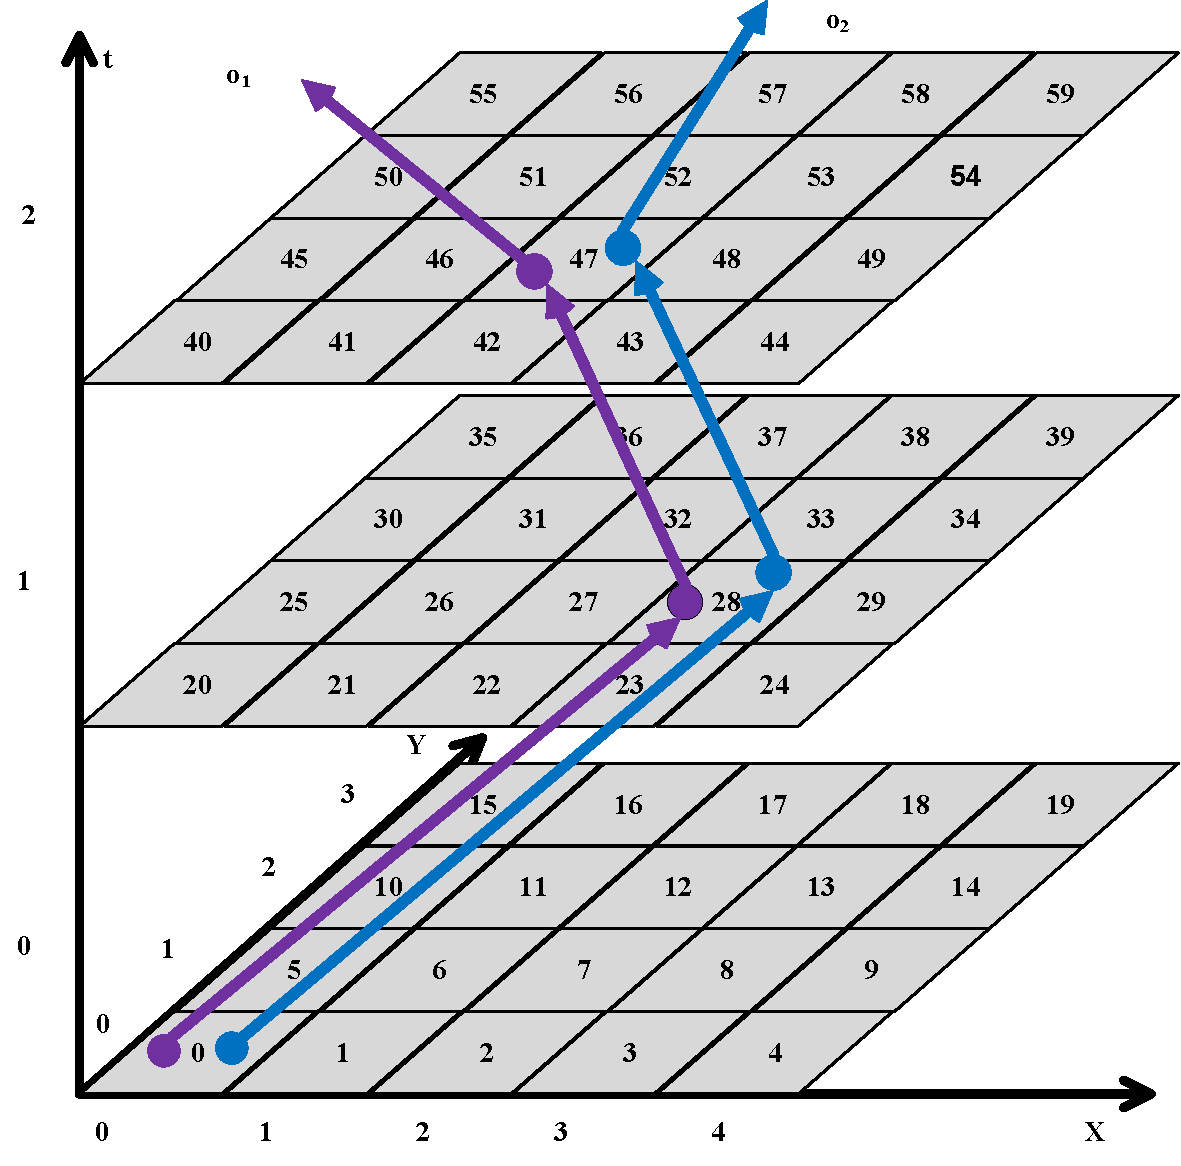
\includegraphics[width=1\textwidth]{fig/section4/picture.pdf}
	\caption{轨迹网格编号及网格编号序列示例}
	\label{cm_fig1:cell_partition}
\end{figure}

\subsubsection{近似协同行为对搜索}

基于轨迹网格编号序列，通过统计两个轨迹之间的公共网格编号数量来近似计算其协同行为持续时间。对于两个轨迹网格编号序列 $O(\tau_i)$ 和 $O(\tau_j)$，若其公共网格编号数 $|O(\tau_i)\cap O(\tau_j)|$ 不小于阈值 $k$，则将 $\langle \tau_i,\tau_j\rangle$ 记录为一个近似协同行为对。该过程对所有轨迹对执行一次，当全部轨迹网格编号序列均被评估完成后终止。

\subsection{社区感知聚类}

对于轨迹集合 $\mathcal{T}=\{\tau_1,\tau_2,\ldots,\tau_{|\mathcal{T}|}\}$，通过第一阶段近似协同行为对搜索后可获得轨迹网格编号序列集合
$O(\mathcal{T})=\{O(\tau_1),O(\tau_2),\ldots,O(\tau_{|\mathcal{T}|})\}$,
以及一组近似协同行为对。在第二阶段中，目标是发现所有满足以下条件的子集 $\mathcal{T}'\subseteq \mathcal{T}$：
(1) $|\mathcal{T}'|\geq m$；
(2) 对任意 $\tau_i,\tau_j\in\mathcal{T}'$，均有 $|O(\tau_i)\cap O(\tau_j)|\geq k$，

即满足伴随群体定义的对象集合。为此，采用聚类技术以实现高效检测。现有轨迹聚类方法主要包括基于划分的聚类 \cite{DBLP:conf/icdm/PelekisKKFT09,DBLP:conf/sigmod/LeeHW07}、基于密度的聚类 \cite{DBLP:conf/dasfaa/LiLLH10,DBLP:journals/access/LiLWYLX18} 以及基于深度学习的聚类 \cite{DBLP:conf/icde/LiZCJW18,DBLP:conf/icws/Zhang0LL019,DBLP:conf/icde/YaoCZB19}。然而，这些方法通常侧重于整体轨迹相似性建模，难以刻画对象之间的显式协同行为连接关系；同时，部分基于密度的方法在大规模数据上具有较高的计算开销。因此，上述针对轨迹聚类或表示学习提出的解决方案，均无法直接应用于本文所研究的伴随群体发现问题。其根本原因在于，聚类方法关注的
是整体轨迹相似度或嵌入空间中的距离关系，而处于同一聚类中的移动对象并不
一定在具体时间段内真实地满足时空共现约束。换言之，轨迹在全局层面上的相
似性并不能保证其在局部时间区间内存在持续的联合移动行为。因此，伴随群体
发现问题仍需基于严格的时空约束建模与结构化搜索策略进行专门设计，而不能
简单依赖现有的轨迹表示学习或聚类方法。

核心思想是将协同行为关系建模为网络（图）结构，其中节点表示移动对象，边表示近似协同行为对。一个伴随群体对应于图中由至少 $m$ 个节点构成的高度结构化子图，且任意两节点之间均满足协同行为约束。受同质性假设的启发——即共享大量协同行为邻居的对象更可能属于同一群体——采用基于共享邻居结构的社区感知聚类方法进行检测。SCAN 算法 \cite{DBLP:conf/kdd/XuYFS07} 是一种典型的社区感知聚类方法，其基于顶点结构相似性与连通性进行社区划分，时间复杂度为 $O(|P|)$，其中 $|P|$ 为协同行为对的数量（即图中的边数）。因此，SCAN 能够高效地应用于伴随群体检测任务。

\begin{theorem}
CS-ACMC 算法的时间复杂度为 $O(|\mathcal{T}|^2 \times |\tau|)$，其中 $|\mathcal{T}|$ 表示轨迹数量，$|\tau|$ 表示单条轨迹的长度。
\end{theorem}

\begin{proof}
在近似协同行为对搜索阶段，需要对每一对轨迹计算其公共网格编号数。若每条轨迹的网格编号序列长度为 $|\tau|$，则通过线性扫描或哈希统计可在 $O(|\tau|)$ 时间内完成一对轨迹的公共网格编号计算。因此，该阶段的时间复杂度为
$
O(|\mathcal{T}|^2 \times |\tau|)
$。在社区感知聚类阶段，SCAN 算法的时间复杂度为 $O(|P|)$，其中 $|P|$ 为近似协同行为对数量，且 $|P|\leq |\mathcal{T}|^2$。因此，整体时间复杂度为
$
O(|\mathcal{T}|^2 \times |\tau| + |P|)=O(|\mathcal{T}|^2 \times |\tau|)
$。综上，CS-ACMC 算法的总体时间复杂度为 $O(|\mathcal{T}|^2 \times |\tau|)$。
\end{proof}

\section{实验评估}
\label{cm_sec:exp}
在本节中，首先介绍实验设定，包括所使用的数据集与运行环境；随后给出实验结果与分析。实验主要关注所提出搜索算法在运行时间方面的表现，即高效性。通过设置不同参数，如轨迹长度、位置点密度、协同行为持续时间阈值等，对比不同算法的运行时间并进行分析。

\subsection{实验设置}

\subsubsection{数据准备}
本文实验基于两个真实世界的出租车轨迹数据集：北京出租车轨迹数据集~\cite{DBLP:conf/kdd/YuanZXS11,DBLP:conf/gis/YuanZZXXSH10}\footnote{https://www.microsoft.com/en-us/research/publication/t-drive-trajectory-data-sample/}以及波尔图出租车轨迹数据集~\footnote{https://www.kaggle.com/c/pkdd-15-predict-taxi-service-trajectory-i/data}。
\paragraph{北京出租车轨迹数据集}
该数据集记录了2008年2月2日至2008年2月8日期间，北京市10357辆出租车的GPS轨迹数据。该数据集包含了约1500万条轨迹点，总距离达到900万公里，平均采样间隔约为177秒，距离约为623米。每个文件以出租车ID命名，详细记录了时间、经度和纬度信息，为城市交通分析、出租车轨迹预测、路径规划以及地理信息系统研究提供了丰富的数据支持。
\paragraph{波尔图出租车轨迹数据集}
本研究采用的波尔图出租车轨迹数据集来源于葡萄牙波尔图市的出租车调度系统。时间跨度为 19 个月，包含超过 170 万条出租车轨迹。所有车辆均通过安装在车载终端中的移动数据设备与调度中心通信，因此能够连续采集高精度 GPS 轨迹数据。该数据集具有时间跨度长、采样频率稳定、轨迹覆盖范围广等特点，能够真实反映城市尺度下出租车群体的动态出行行为，为协同行为模式挖掘与群体结构分析提供了可靠的数据基础。

\paragraph{数据预处理}

为统一实验设定，所有时间戳均被映射到 24 小时范围内。对于波尔图数据集，每条轨迹的出发时间被随机分配至 24 小时区间内，以避免时间分布偏置。所有轨迹数据在实验前均被预处理并转换为轨迹网格编号序列。生成网格编号序列及伴随群体发现所使用的默认参数设置如表 \ref{cm_tb: group settings} 所示。同时，对轨迹的经纬度范围以及轨迹长度进行了筛选与限制，以保证实验规模可控且具有代表性，具体参数同样列于表 \ref{cm_tb: group settings} 中。

\begin{table}[tb]
	\centering
	\caption{参数设定}
	\label{cm_tb: group settings}
	\begin{tabular}{|l|l|l|}
		\hline
		\bfseries & \bfseries 北京数据集  & \bfseries 波尔图数据集 \\
		\hline
		\hline
		经度范围  & \tabincell{l}{[116.250, 116.550]} &  \tabincell{l}{[-8.735, -8.156]} \\
		\hline
		维度范围  & \tabincell{l}{[39.830,  40.030]}& \tabincell{l}{[40.953, 41.307]} \\
		\hline
		轨迹长度范围  & \tabincell{l}{[20, 100]}& \tabincell{l}{[20, 100]} \\
		\hline
		\tabincell{l}{$\epsilon_s$} & \tabincell{l}{200 米} &  \tabincell{l}{200 米} \\
  \hline
		\tabincell{l}{$\epsilon_t$} & \tabincell{l}{200 秒} &  \tabincell{l}{200 秒} \\
  \hline
		$|\mathcal{T}|$ & \tabincell{l}{2K--10K / 默认 6K}& \tabincell{l}{20K--100K / 默认 20K} \\
		\hline
  $k$ & \tabincell{l}{2--6 / 默认 4}& \tabincell{l}{2--6 / 默认 4} \\
		\hline
		 $m$ & \tabincell{l}{2--6 / 默认 4}& \tabincell{l}{2--6 /默认 4} \\
   \hline
   $\mu$ & \tabincell{l}{0.42--0.50 / 默认 0.50}& \tabincell{l}{0.42--0.50 / 默认 0.50} \\
		\hline
	\end{tabular}
\end{table}
    

\subsubsection{比较算法}

\begin{table}[htbp]
    \centering
    \setlength{\tabcolsep}{8pt}% column separation
    \caption{比较算法}
    \label{cm_tab:compared_alg}
    \renewcommand{\arraystretch}{1}%row space 
    \begin{tabular}{ll}
        \hline
		\bfseries 算法标识 & \bfseries 算法描述 \\
        \hline
        ES-ECMC & 精确搜索算法\\
        CS-ACMC & 基于近似协同行为计算的社区感知搜索算法 \\ 
        \hline
    \end{tabular}
\end{table}

表\ref{cm_tab:compared_alg}列举了实验研究中的比较算法。
本文对以下两种算法进行性能比较：ES-ECMC算法，以及CS-ACMC算法。
此外，在候选对象筛选阶段引入R树索引结构 \cite{DBLP:conf/sigmod/Guttman84}，以对空间上显然不满足距离约束的对象对进行早期剪枝，从而减少无效距离计算并提升整体运行效率。

\subsubsection{评估指标}

为了评估 CS-ACMC 算法的有效性，采用 ES-ECMC 算法所发现的精确协同行为对作为基准，并使用协同行为对的平均命中率作为主要质量评估指标。具体而言，对于 ES-ECMC 算法发现的每一个精确伴随群体 $g$，若其中任意一个协同行为对 $\langle o_i,o_j\rangle$（其中 $o_i\in g, o_j\in g$）同时存在于 CS-ACMC 算法所发现的任意一个伴随群体中，则认为该协同行为对被命中，命中计数加一；否则认为未被命中。最终统计所有精确协同行为对的命中比例，作为整体命中率。该指标能够有效反映近似算法在保持协同行为结构方面的结果质量。在效率评估方面，采用平均 CPU 运行时间作为主要性能指标。需要说明的是，在默认参数设置下，ES-ECMC 算法在北京数据集上采用单线程运行时至少需要 1 天时间，因此实验中为 ES-ECMC 启用了 40 个线程以保证实验可行性；相比之下，CS-ACMC 算法仅使用单线程运行。

\subsubsection{实验环境}
所有算法均采用 Python 实现，并运行于 Ubuntu 操作系统平台。实验硬件环境为：2 颗 Intel(R) Xeon(R) Silver 4214R CPU（主频 2.40GHz）以及 128GB 内存。除非特别说明，所有实验结果均为在 20 组不同测试轨迹输入下重复实验所得的平均值，以减少偶然因素对结果的影响。

\subsection{实验结果与分析}

\subsubsection{轨迹数量的影响}

首先，在默认参数设置下，研究轨迹数量变化对算法性能的影响。具体而言，在波尔图数据集中，轨迹数量从 20{,}000 增加至 100{,}000；在北京数据集中，轨迹数量从 2{,}000 增加至 10{,}000。之所以采用该设置，是因为北京数据集的轨迹空间分布更加密集、采样间隔更小，因此任意两条轨迹更容易满足距离约束并形成协同行为对，从而带来更高的计算压力。从命中率结果来看，波尔图数据集上的命中率随轨迹数量增加呈现明显上升趋势（见图~\ref{cm_fig:波尔图数据集-ratios-num}）。当轨迹数量由 20K 增加至 100K 时，命中率由约 0.70 提升至接近 0.88。这一现象说明，在轨迹规模较小时，近似方法可能因协同行为对数量较少而遗漏部分结构；随着轨迹数量增加，对象之间的连接关系更加充分，社区结构更加清晰，基于共享邻居的聚类策略能够更准确地恢复真实伴随群体结构。相比之下，北京数据集上的命中率始终稳定在 0.91--0.93 之间（见图~\ref{cm_fig:北京数据集-ratios-num}），整体波动较小。这是因为北京数据集本身轨迹密度较高，在较小规模下已能形成相对稳定的协同行为图结构，因此随着规模增加，近似算法的结果质量提升空间有限，但整体保持较高水平。

\begin{figure}[htbp]
    \centering
    \subfloat[]{
        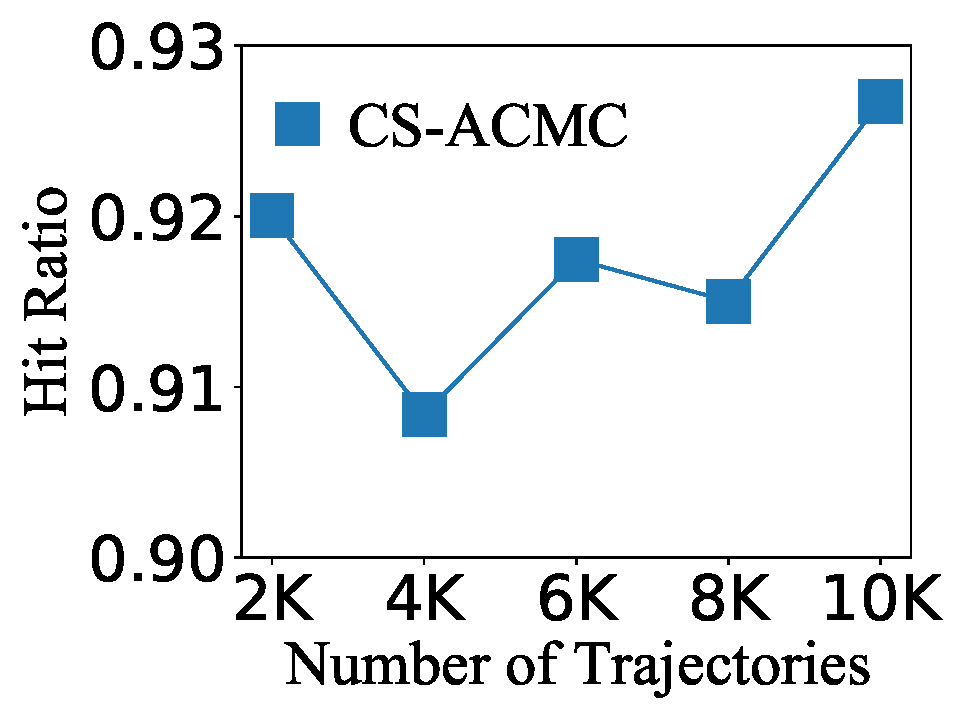
\includegraphics[width=0.4\textwidth]{fig/section4/BJ-hitratio-num.pdf}
        \label{cm_fig:北京数据集-ratios-num}
    }
    \hfill
    \subfloat[]{
        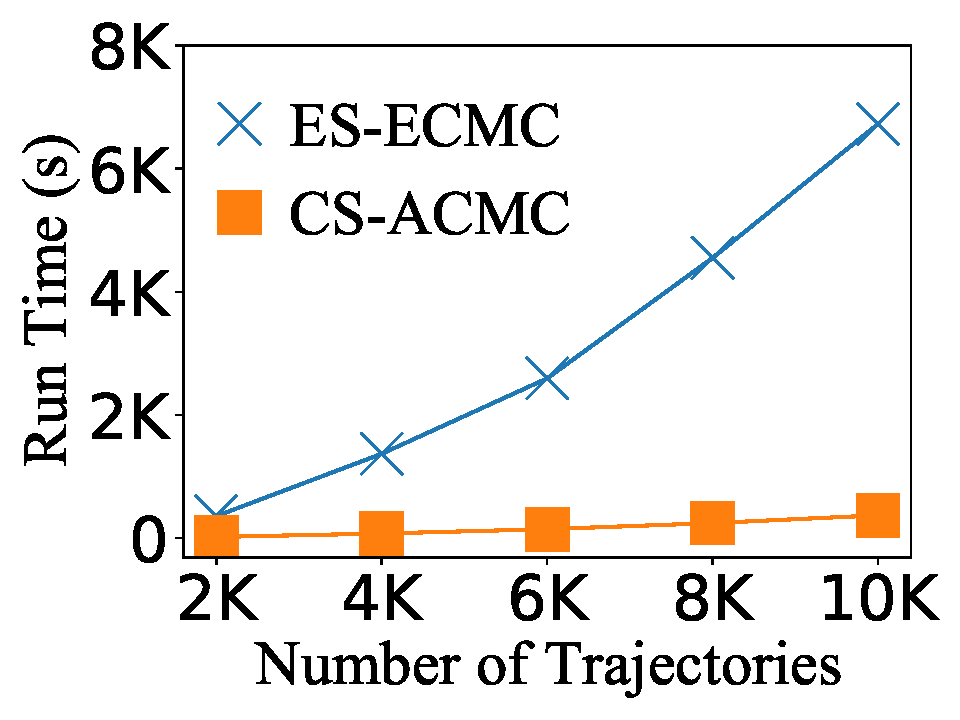
\includegraphics[width=0.4\textwidth]{fig/section4/BJ-time-num.pdf}
        \label{cm_fig:北京数据集-time-num}
    }
    \\
    \subfloat[]{
        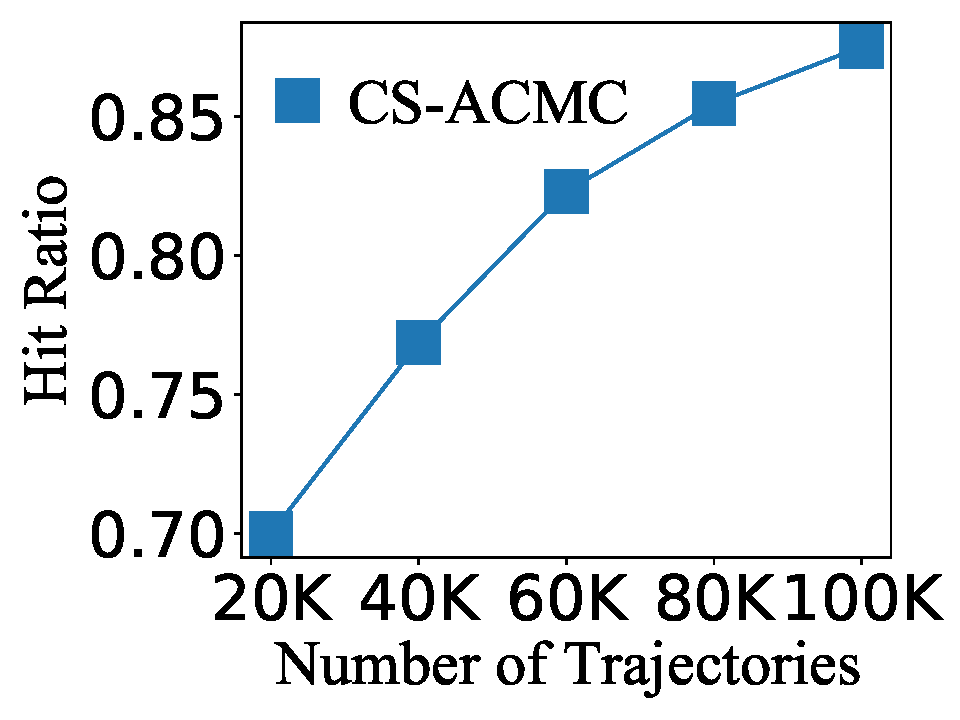
\includegraphics[width=0.4\textwidth]{fig/section4/PT-hitratio-num.pdf}
        \label{cm_fig:波尔图数据集-ratios-num}
    }
    \hfill
    \subfloat[]{
        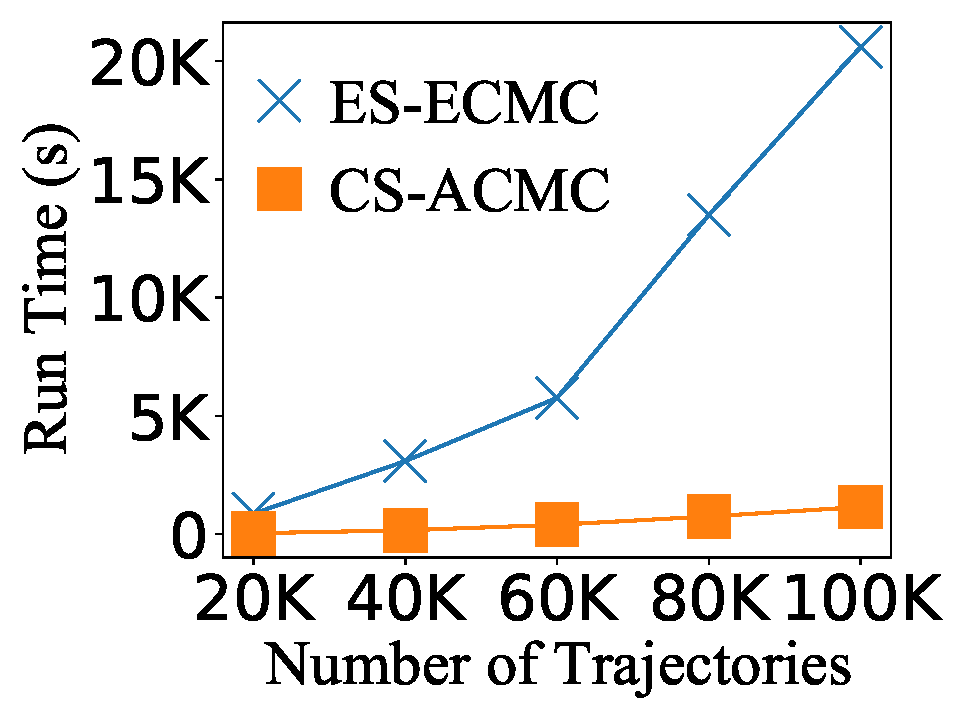
\includegraphics[width=0.4\textwidth]{fig/section4/PT-time-num.pdf}
        \label{cm_fig:波尔图数据集-time-num}
    }
    \caption{轨迹数量的影响。 \subref{cm_fig:北京数据集-ratios-num} 北京数据集上的命中率 \subref{cm_fig:北京数据集-time-num} 北京数据集上的运行时间 \subref{cm_fig:波尔图数据集-ratios-num} 波尔图数据集上的命中率 \subref{cm_fig:波尔图数据集-time-num} 波尔图数据集上的运行时间}
	\label{cm_fig:trjNum}
\end{figure}


在算法运行效率方面，两种算法的运行时间均随轨迹数量增加而增长，但增长趋势存在显著差异。ES-ECMC 的运行时间随规模增加呈现近似二次增长趋势；而 CS-ACMC 的增长速度明显更缓（见图~\ref{cm_fig:北京数据集-time-num} 和图~\ref{cm_fig:波尔图数据集-time-num}）。即便 ES-ECMC 在实验中采用了 40 线程并行计算，当轨迹数量达到 10{,}000（北京）和 100{,}000（波尔图数据集）时，其运行时间仍分别超过 8{,}000 秒和 20{,}000 秒；相比之下，CS-ACMC 在单线程条件下的运行时间始终控制在千秒以内。值得注意的是，波尔图数据集中捕获的协同行为对数量明显多于北京数据集，导致图结构更加稠密，从而增加了精确算法的计算负担。这也进一步放大了两种方法在大规模场景下的性能差距。综上所述，随着轨迹数量的增加，CS-ACMC 在保证较高命中率（尤其在大规模数据上不断提升）的同时，始终保持至少一个数量级的时间优势。这表明该方法在大规模轨迹数据分析场景下具有良好的可扩展性和实际应用价值。


\subsubsection{协同行为持续时间阈值的影响}
\begin{figure}
    \centering
    \subfloat[]{ 
        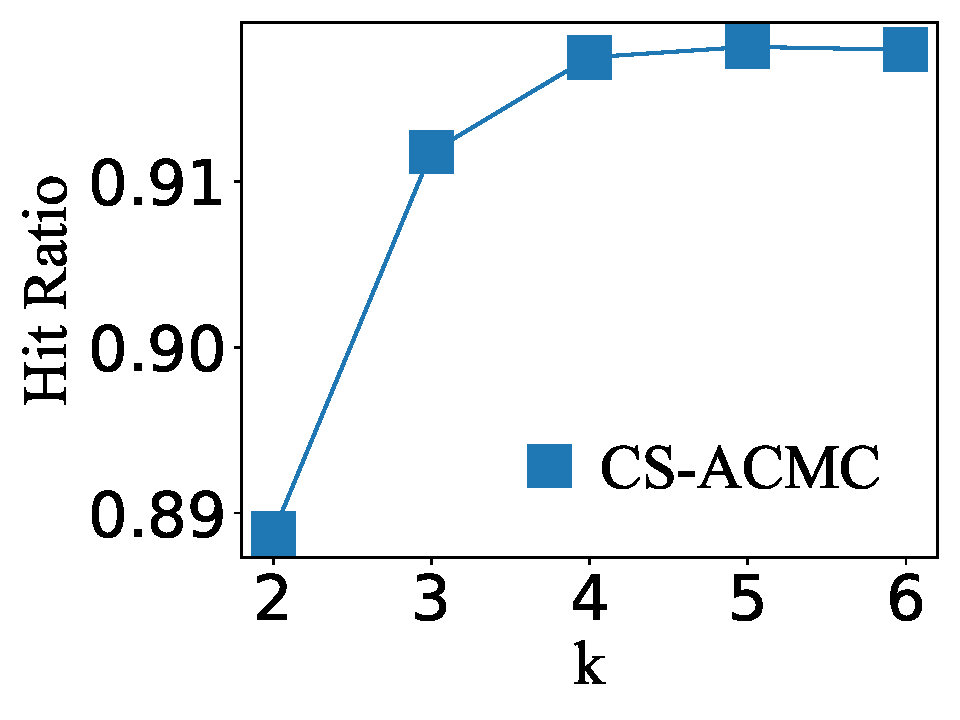
\includegraphics[width=0.4\textwidth]{fig/section4/BJ-hitratio-k.pdf}
        \label{cm_fig:北京数据集-ratios-k}
    }
    \hfill
    \subfloat[]{
        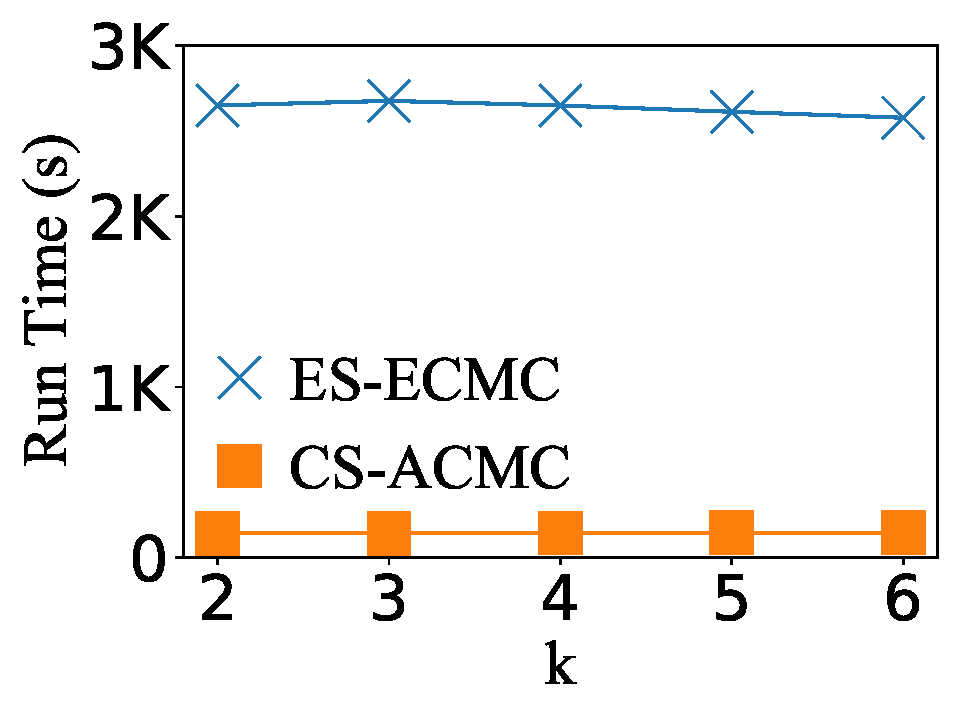
\includegraphics[width=0.4\textwidth]{fig/section4/BJ-time-k.pdf}
        \label{cm_fig:北京数据集-time-k}
    }
    \\
    \subfloat[]{
        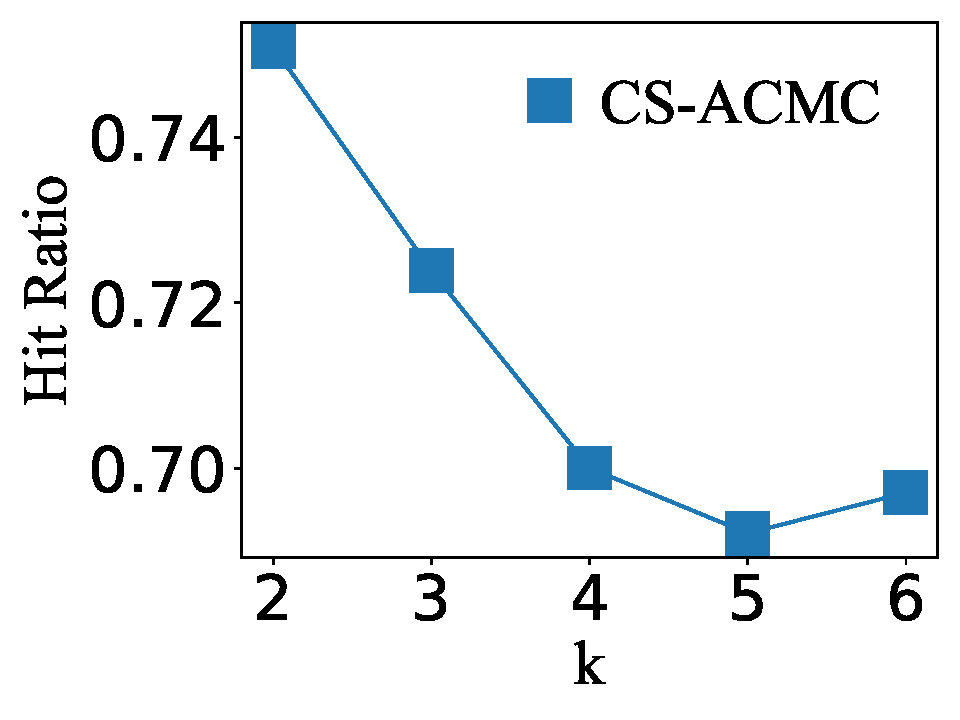
\includegraphics[width=0.4\textwidth]{fig/section4/PT-hitratio-k.pdf}
        \label{cm_fig:波尔图数据集-ratios-k}
    }
    \hfill
    \subfloat[]{
        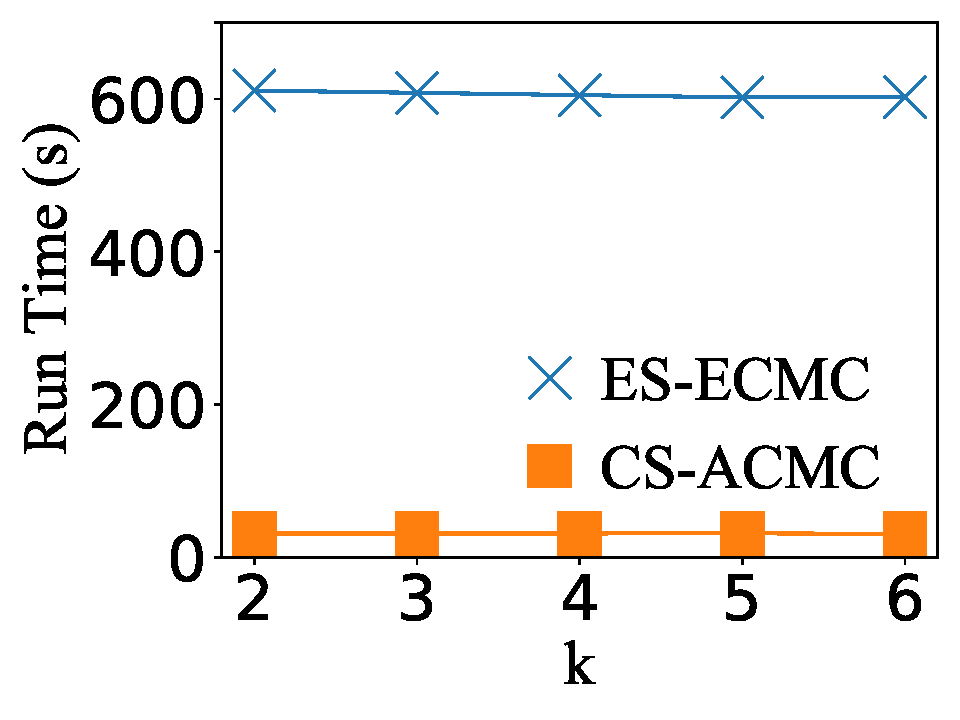
\includegraphics[width=0.4\textwidth]{fig/section4/PT-time-k.pdf}
        \label{cm_fig:波尔图数据集-time-k}
    }
    \caption{协同行为持续时间阈值的影响。\subref{cm_fig:北京数据集-ratios-k} 北京数据集上的命中率 \subref{cm_fig:北京数据集-time-k} 北京数据集上的运行时间 \subref{cm_fig:波尔图数据集-ratios-k} 波尔图数据集上的命中率 \subref{cm_fig:波尔图数据集-time-k} 波尔图数据集上的运行时间}
\label{cm_fig:k}
\end{figure}

图 \ref{cm_fig:k} 展示了当协同行为持续时间阈值 $k$ 从 2 增加到 6 时两种算法的性能变化趋势。
从命中率角度来看，北京数据集上的命中率随 $k$ 增大呈现缓慢上升趋势（见图~\ref{cm_fig:北京数据集-ratios-k}）。当 $k=2$ 时命中率约为 0.89，随后逐步提升并稳定在 0.91 以上。这表明在北京这种高密度轨迹环境下，提高持续时间阈值能够有效过滤掉短暂、偶然的协同行为，使近似方法更聚焦于结构稳定的协同行为对，从而提升结果质量。相比之下，波尔图数据集上的命中率随着 $k$ 的增大整体呈下降趋势（见图~\ref{cm_fig:波尔图数据集-ratios-k}），从约 0.75 下降至 0.69 左右。这是因为波尔图数据集采样频率更高、时间跨度更长，较大的 $k$ 会显著减少满足条件的协同行为对数量，使得图结构变得稀疏，进而影响基于共享邻居的社区识别效果。因此，近似方法在较大 $k$ 下更容易遗漏部分真实协同行为结构。

在运行时间方面，如图~\ref{cm_fig:北京数据集-time-k} 和图~\ref{cm_fig:波尔图数据集-time-k}，两种算法均未随着 $k$ 的增大而出现明显下降趋势。尽管理论上更大的 $k$ 会减少协同行为对及伴随群体数量，从而降低后续聚类成本，但实验结果表明，总体运行时间基本保持稳定。其主要原因在于，算法的核心计算开销集中在协同行为对的枚举或近似计算阶段，而该阶段需要对所有轨迹对进行比较，其复杂度与 $k$ 无关；从协同行为对中生成伴随群体的代价相对较低，因此 $k$ 的变化对总时间影响有限。同时可以观察到，在所有 $k$ 取值下，CS-ACMC 的运行时间始终显著低于 ES-ECMC。即使在较小 $k$（的情况下，CS-ACMC 仍保持明显的效率优势，进一步验证了近似计算策略在降低计算成本方面的有效性。

\subsubsection{群体规模阈值的影响}

图 \ref{cm_fig:m} 展示了当群体规模阈值 $m$ 从 2 变化到 6 时两种算法性能的变化趋势。直觉上，随着 $m$ 的增大，满足条件的伴随群体数量逐渐减少，因为只有结构更加紧密、连接更加稳定的对象集合才能满足更严格的规模约束。这一变化对结果质量与运行时间均产生一定影响。如图~\ref{cm_fig:北京数据集-ratios-m}，北京数据集上的命中率随着 $m$ 的增加呈显著上升趋势。当 $m=2$ 时命中率约为 0.71，而当 $m=5$ 或 $6$ 时可提升至 0.93 左右。这说明在高密度轨迹环境下，小规模群体中包含较多边界性或弱连接结构，近似方法可能存在一定偏差；而当 $m$ 增大后，仅保留结构更加紧密的核心群体，使得近似方法与精确方法在识别结果上更加一致，从而显著提升命中率。相比之下，波尔图数据集上的命中率随着 $m$ 的增加呈下降趋势，从约 0.88 下降至 0.59 左右。这主要是由于波尔图数据集数据的空间分布更为分散、轨迹时间跨度更长。当 $m$ 较大时，满足条件的群体数量显著减少，图结构趋于稀疏，近似协同行为对可能无法完整保留所有真实连接关系，导致部分精确群体未被成功恢复，从而降低命中率。

在效率方面（见图~\ref{cm_fig:北京数据集-time-m} 和图~\ref{cm_fig:波尔图数据集-time-m}），群体规模阈值 $m$ 的变化对总体运行时间影响较小。两种算法的运行时间曲线基本保持平稳，仅在个别取值处存在轻微波动。这进一步验证了前文分析：算法的主要时间开销集中在协同行为对的构建或近似计算阶段，而最终伴随群体的筛选与过滤成本相对较低，因此 $m$ 的变化不会显著改变总体时间复杂度。
同时可以观察到，在所有 $m$ 取值下，CS-ACMC 的运行时间始终远低于 ES-ECMC。即使在波尔图数据集中，当 $m=6$ 时 ES-ECMC 的运行时间超过 8{,}000 秒，而 CS-ACMC 仍保持在数百秒以内，体现出明显的规模优势。
综上所述，在不同 $m$ 参数设置下，CS-ACMC 在保持较高命中率（尤其在高密度数据集上）的同时，显著降低了运行时间，表现出良好的稳定性与参数鲁棒性。这表明该方法能够适应不同规模约束条件，在多种实际应用场景中具有较强的实用价值。


\begin{figure}[htbp]
    \centering
    \subfloat[]{
        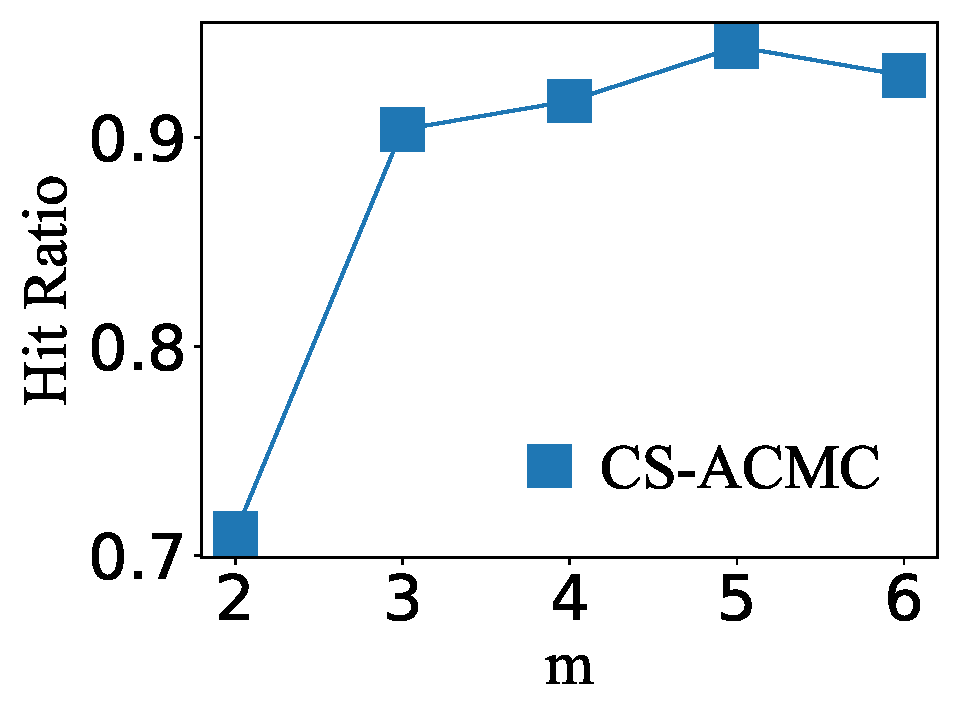
\includegraphics[width=0.4\textwidth]{fig/section4/BJ-hitratio-m.pdf}
        \label{cm_fig:北京数据集-ratios-m}
    }
    \hfill
    \subfloat[]{
        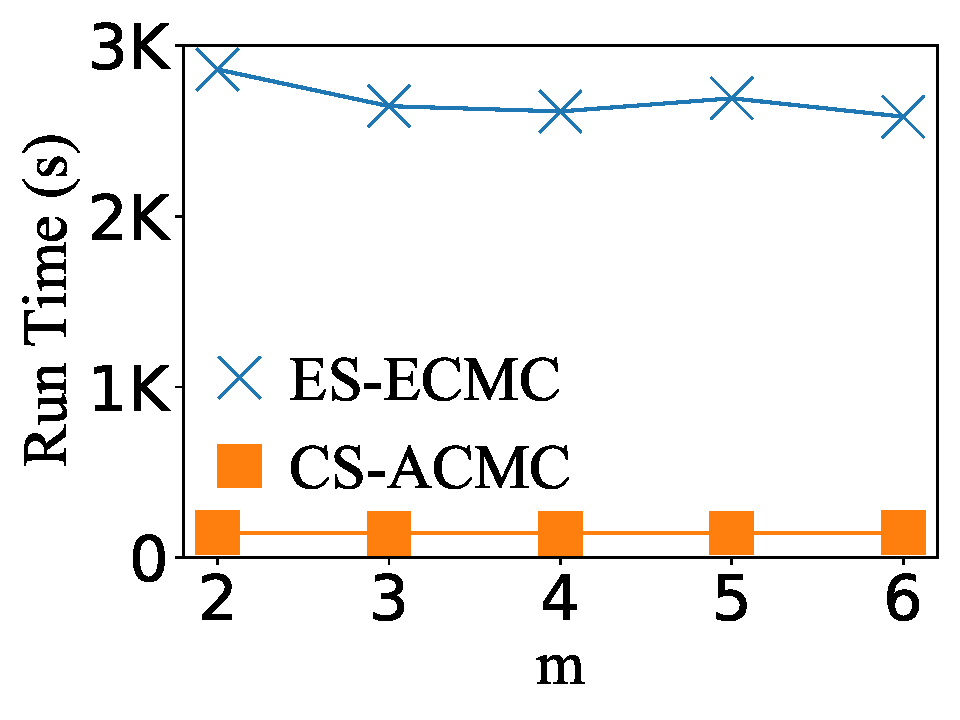
\includegraphics[width=0.4\textwidth]{fig/section4/BJ-time-m.pdf}
        \label{cm_fig:北京数据集-time-m}
    }
    \\
    \subfloat[]{
        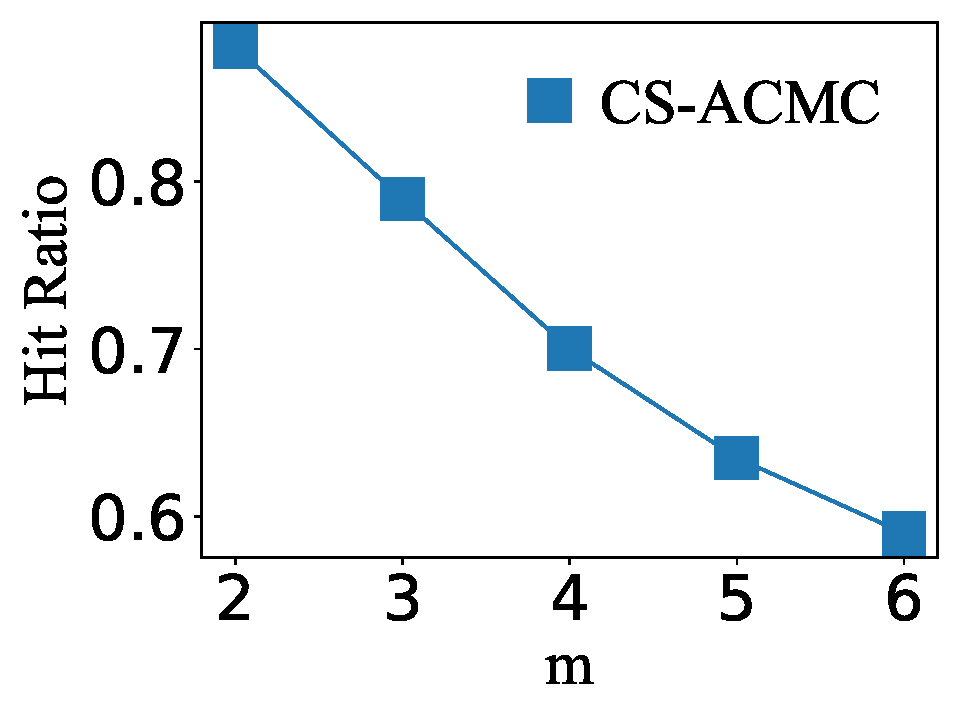
\includegraphics[width=0.4\textwidth]{fig/section4/PT-hitratio-m.pdf}
        \label{cm_fig:波尔图数据集-ratios-m}
    }
    \hfill
    \subfloat[]{
        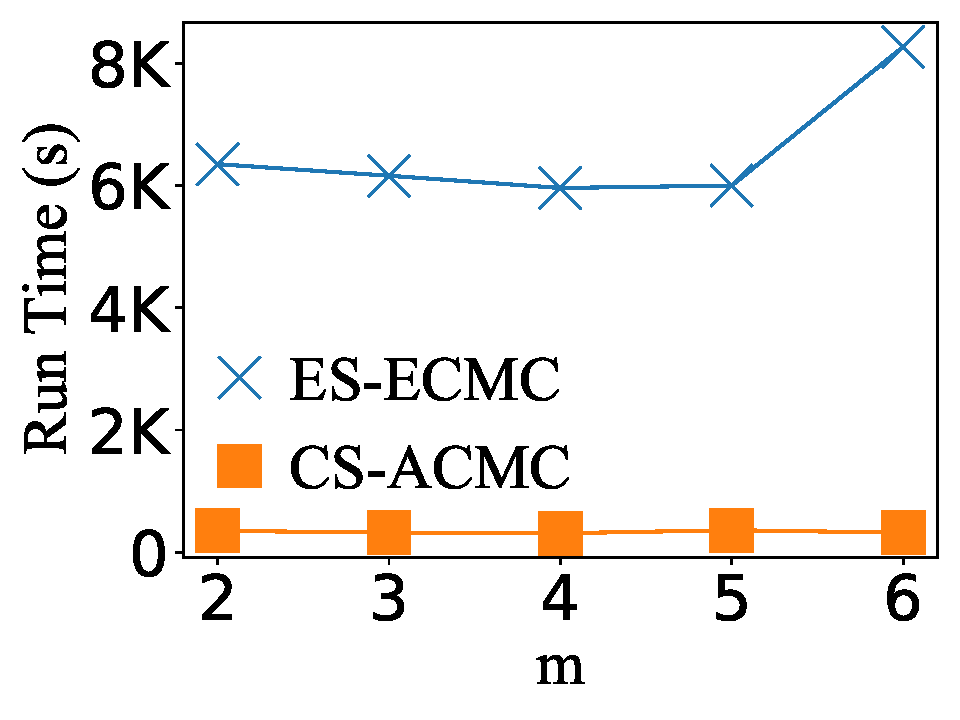
\includegraphics[width=0.4\textwidth]{fig/section4/PT-time-m.pdf}
        \label{cm_fig:波尔图数据集-time-m}
    }
    \caption{群体规模阈值的影响。\subref{cm_fig:北京数据集-ratios-m} 北京数据集上的命中率 \subref{cm_fig:北京数据集-time-m} 北京数据集上的运行时间 \subref{cm_fig:波尔图数据集-ratios-m} 波尔图数据集上的命中率 \subref{cm_fig:波尔图数据集-time-m} 波尔图数据集上的运行时间}
    \label{cm_fig:m}
\end{figure}


\subsubsection{聚类参数的影响}
\begin{figure}[htbp]
    \centering
    \subfloat[]{
        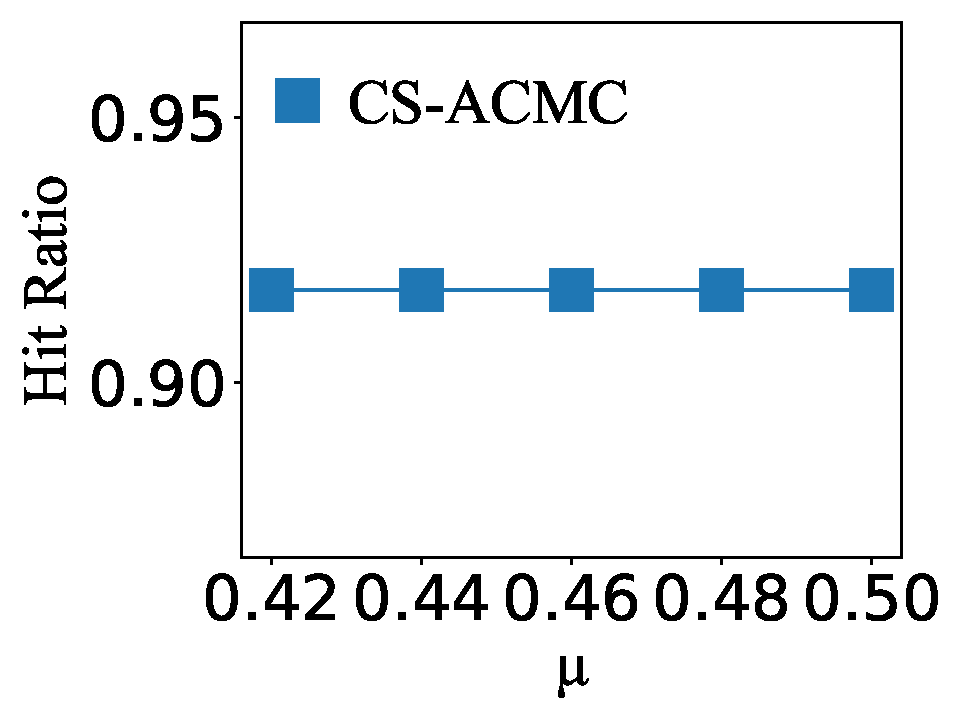
\includegraphics[width=0.4\textwidth]{fig/section4/BJ-hitratio-ep.pdf}
        \label{cm_fig:北京数据集-ratios-ep}
    }
    \hfill
    \subfloat[]{
        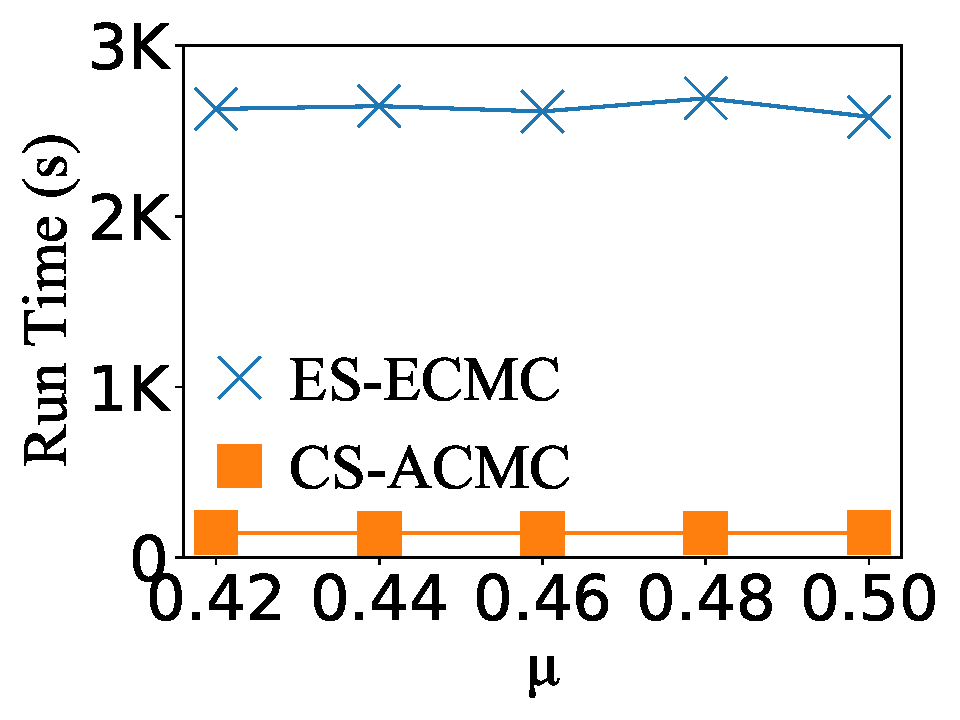
\includegraphics[width=0.4\textwidth]{fig/section4/BJ-time-ep.pdf}
        \label{cm_fig:北京数据集-time-ep}
    }

    \subfloat[]{
        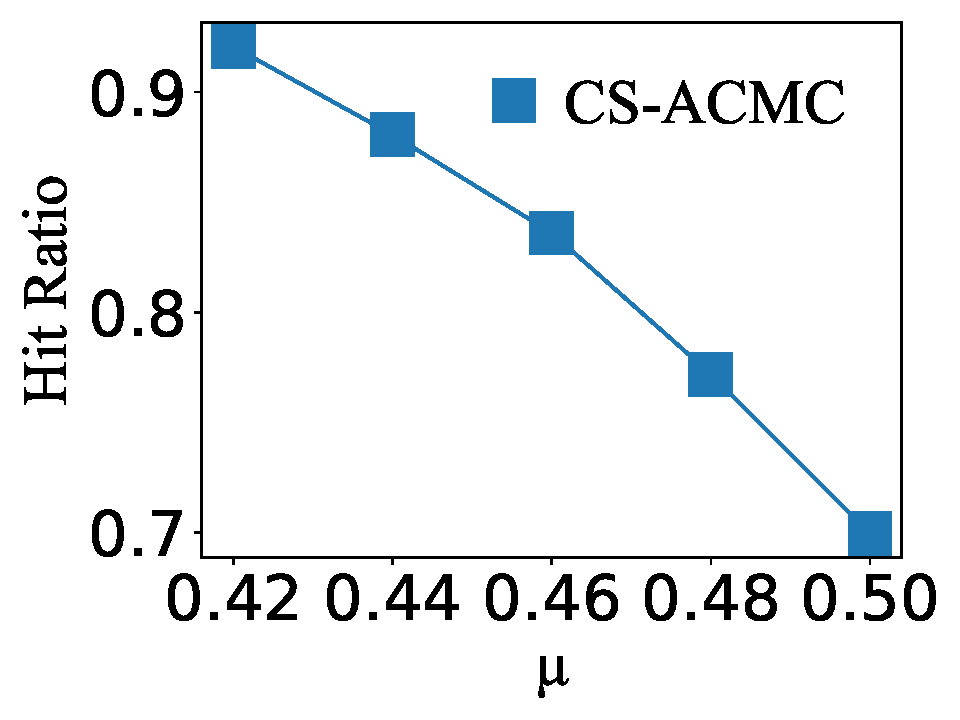
\includegraphics[width=0.4\textwidth]{fig/section4/PT-hitratio-ep.pdf}
        \label{cm_fig:波尔图数据集-ratios-ep}
    }
    \hfill
    \subfloat[]{
        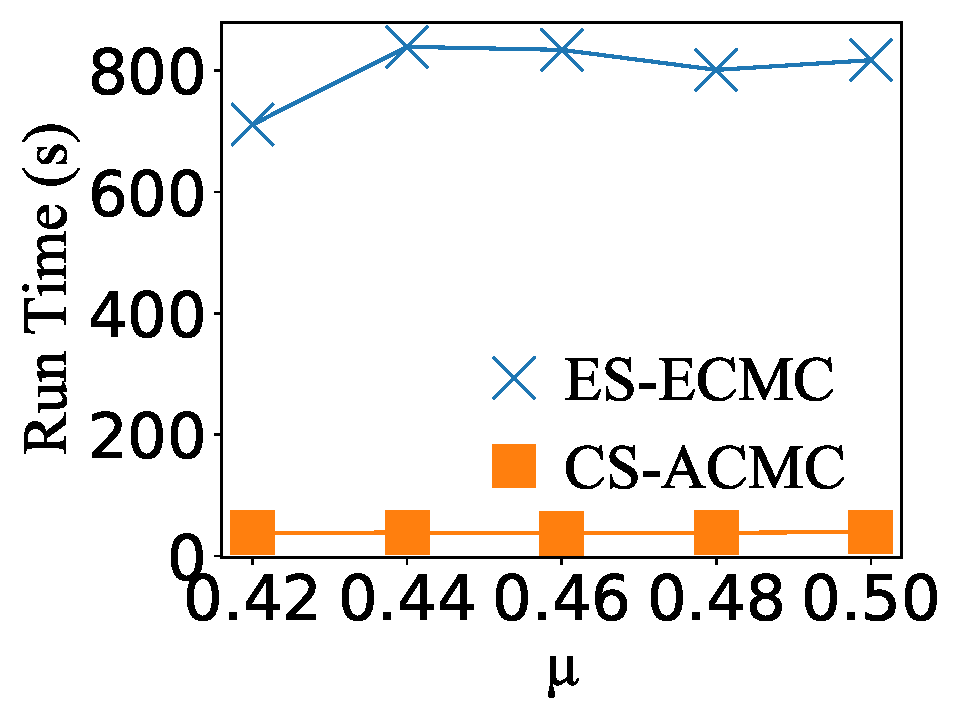
\includegraphics[width=0.4\textwidth]{fig/section4/PT-time-ep.pdf}
        \label{cm_fig:波尔图数据集-time-ep}
    }
    \caption{SCAN聚类结构相似度参数的影响。\subref{cm_fig:北京数据集-ratios-ep} 北京数据集上的命中率 \subref{cm_fig:北京数据集-time-ep} 北京数据集上的运行时间 \subref{cm_fig:波尔图数据集-ratios-ep} 波尔图数据集上的命中率 \subref{cm_fig:波尔图数据集-time-ep} 波尔图数据集上的运行时间}
    \label{cm_fig:ep}
\end{figure}


图 \ref{cm_fig:ep} 展示了当结构相似度阈值 $\mu$ 从 0.42 增加到 0.50 时算法在两个数据集上的命中率与运行时间变化情况。结构相似度阈值用于控制对象之间是否建立连接：$\mu$ 越小，两个对象越容易满足相似性条件，从而在协同行为图中形成更多边；$\mu$ 越大，则连接关系更加严格，图结构趋于稀疏。

从命中率变化趋势来看，在波尔图数据集中（见图~\ref{cm_fig:波尔图数据集-ratios-ep}），随着 $\mu$ 的增大，命中率呈现明显下降趋势。当 $\mu=0.42$ 时取得最佳效果，而当 $\mu=0.50$ 时命中率下降至约 0.70。这表明在空间分布较为分散的数据环境下，适当放宽结构相似度约束有助于保留潜在的真实连接关系，而过高的阈值会导致部分真实协同关系被过滤，进而影响整体命中率。相比之下，北京数据集上的命中率始终稳定在 0.91 以上，且随 $\mu$ 的变化波动较小（见图~\ref{cm_fig:北京数据集-ratios-ep}）。这一现象主要归因于北京数据集更高的轨迹采样密度和更强的空间聚集性。在高密度环境中，即使提高相似度阈值，真实协同行为之间仍能保持较高的结构一致性，因此算法结果对 $\mu$ 的敏感度较低，表现出更强的稳定性。

在效率方面（见图~\ref{cm_fig:北京数据集-time-ep} 和图~\ref{cm_fig:波尔图数据集-time-ep}），两种算法的运行时间均未随 $\mu$ 的变化出现显著波动，说明结构相似度阈值主要影响图的连接密度，而对整体计算流程的复杂度影响有限。然而，即便 ES-ECMC 采用多线程实现，其运行时间仍显著高于 CS-ACMC，在两个数据集上均至少相差一个数量级。这表明本文提出的近似协同行为构建策略在降低候选连接数量的同时，有效控制了计算开销。

\section{本章小结}
\label{cm_sec:conclusion}

针对传统协同行为模式定义过于严格、难以适应真实轨迹数据中噪声与不规则性的不足，提出了一种放宽的协同行为模式定义，在保证语义合理性的同时，提高了模型对实际数据的适应能力。

从数据处理模式的角度来看，现有方法可大致分为静态处理与流式处理两类。一些方法（如~\cite{DBLP:conf/icde/ZhengZYS13,DBLP:journals/tkde/ZhengZYSZ14,DBLP:conf/sigmod/FangGPCMJ20}）能够处理轨迹数据流，支持持续更新与在线检测；而另一些方法则主要面向离线或静态轨迹数据（如~\cite{DBLP:conf/gis/VieiraBT09,DBLP:journals/pvldb/JeungYZJS08,DBLP:journals/pvldb/LiDHK10}）。与本文最为相关的工作之一是 Chen 等人~\cite{DBLP:journals/pvldb/ChenGFMJG19} 提出的实时联合移动模式挖掘方法。该方法定义了一种更为通用的联合移动模式，并通过 $L$-连续性与 $G$-连通性刻画轨迹之间的时间连续性与结构连通性。然而，由于问题定义存在本质差异，该方法无法直接应用于本文场景：一方面，本文不要求时间上的严格连续性或连通性；另一方面，也不要求对象在每个时间点均属于同一聚类结构；此外，当一个对象能够参与多个群体时，本文采用“成员规模最大优先”的归属策略，以保证结果的确定性与可解释性。

围绕上述问题，分别设计了精确算法与近似算法。精确算法通过完整枚举与严格验证协同行为对，能够获得理论上的最优结果，但在大规模数据场景下面临较高的时间复杂度。为此，进一步提出了基于结构剪枝与候选压缩策略的近似算法，通过构建紧凑的协同行为图结构，有效减少冗余计算与无效候选，从而在保证较高命中率的前提下显著降低运行开销。两种算法在设计思路上相互补充：前者保证结果精确性，后者强调规模可扩展性，共同构成了完整的解决方案体系。

在实验评估方面，基于北京与波尔图数据集两个真实世界轨迹数据集，从轨迹数量、协同行为持续时间阈值 $k$、群体规模阈值 $m$ 以及结构相似度阈值 $\mu$ 等多个维度进行了系统分析。实验结果表明：（1）在不同数据规模下，CS-ACMC 均表现出良好的可扩展性，其运行时间相比 ES-ECMC 至少降低一个数量级；（2）在高密度数据集上，近似算法能够保持稳定且较高的命中率，体现出较强的鲁棒性；（3）参数变化对算法运行时间影响有限，说明主要计算开销集中在协同行为对构建阶段；（4）在不同数据分布特性下，结构相似度与群体规模参数对命中率的影响具有一定差异，进一步验证了方法在多场景下的适应能力。

从应用角度来看，本章研究成果对于交通管理与城市计算具有重要意义。通过对潜在协同行为群体的提前识别，可以辅助分析车队行驶、异常聚集、隐性组织化出行等行为模式，为拥堵预测、路径规划优化以及公共安全监测提供数据支持。同时，所提出的近似建模与剪枝策略也可推广至其他大规模时空模式挖掘任务，具有较强的通用性。

